% Options for packages loaded elsewhere
\PassOptionsToPackage{unicode}{hyperref}
\PassOptionsToPackage{hyphens}{url}
%
\documentclass[
]{article}
\usepackage{amsmath,amssymb}
\usepackage{iftex}
\ifPDFTeX
  \usepackage[T1]{fontenc}
  \usepackage[utf8]{inputenc}
  \usepackage{textcomp} % provide euro and other symbols
\else % if luatex or xetex
  \usepackage{unicode-math} % this also loads fontspec
  \defaultfontfeatures{Scale=MatchLowercase}
  \defaultfontfeatures[\rmfamily]{Ligatures=TeX,Scale=1}
\fi
\usepackage{lmodern}
\ifPDFTeX\else
  % xetex/luatex font selection
\fi
% Use upquote if available, for straight quotes in verbatim environments
\IfFileExists{upquote.sty}{\usepackage{upquote}}{}
\IfFileExists{microtype.sty}{% use microtype if available
  \usepackage[]{microtype}
  \UseMicrotypeSet[protrusion]{basicmath} % disable protrusion for tt fonts
}{}
\makeatletter
\@ifundefined{KOMAClassName}{% if non-KOMA class
  \IfFileExists{parskip.sty}{%
    \usepackage{parskip}
  }{% else
    \setlength{\parindent}{0pt}
    \setlength{\parskip}{6pt plus 2pt minus 1pt}}
}{% if KOMA class
  \KOMAoptions{parskip=half}}
\makeatother
\usepackage{xcolor}
\usepackage[margin=1in]{geometry}
\usepackage{color}
\usepackage{fancyvrb}
\newcommand{\VerbBar}{|}
\newcommand{\VERB}{\Verb[commandchars=\\\{\}]}
\DefineVerbatimEnvironment{Highlighting}{Verbatim}{commandchars=\\\{\}}
% Add ',fontsize=\small' for more characters per line
\usepackage{framed}
\definecolor{shadecolor}{RGB}{248,248,248}
\newenvironment{Shaded}{\begin{snugshade}}{\end{snugshade}}
\newcommand{\AlertTok}[1]{\textcolor[rgb]{0.94,0.16,0.16}{#1}}
\newcommand{\AnnotationTok}[1]{\textcolor[rgb]{0.56,0.35,0.01}{\textbf{\textit{#1}}}}
\newcommand{\AttributeTok}[1]{\textcolor[rgb]{0.13,0.29,0.53}{#1}}
\newcommand{\BaseNTok}[1]{\textcolor[rgb]{0.00,0.00,0.81}{#1}}
\newcommand{\BuiltInTok}[1]{#1}
\newcommand{\CharTok}[1]{\textcolor[rgb]{0.31,0.60,0.02}{#1}}
\newcommand{\CommentTok}[1]{\textcolor[rgb]{0.56,0.35,0.01}{\textit{#1}}}
\newcommand{\CommentVarTok}[1]{\textcolor[rgb]{0.56,0.35,0.01}{\textbf{\textit{#1}}}}
\newcommand{\ConstantTok}[1]{\textcolor[rgb]{0.56,0.35,0.01}{#1}}
\newcommand{\ControlFlowTok}[1]{\textcolor[rgb]{0.13,0.29,0.53}{\textbf{#1}}}
\newcommand{\DataTypeTok}[1]{\textcolor[rgb]{0.13,0.29,0.53}{#1}}
\newcommand{\DecValTok}[1]{\textcolor[rgb]{0.00,0.00,0.81}{#1}}
\newcommand{\DocumentationTok}[1]{\textcolor[rgb]{0.56,0.35,0.01}{\textbf{\textit{#1}}}}
\newcommand{\ErrorTok}[1]{\textcolor[rgb]{0.64,0.00,0.00}{\textbf{#1}}}
\newcommand{\ExtensionTok}[1]{#1}
\newcommand{\FloatTok}[1]{\textcolor[rgb]{0.00,0.00,0.81}{#1}}
\newcommand{\FunctionTok}[1]{\textcolor[rgb]{0.13,0.29,0.53}{\textbf{#1}}}
\newcommand{\ImportTok}[1]{#1}
\newcommand{\InformationTok}[1]{\textcolor[rgb]{0.56,0.35,0.01}{\textbf{\textit{#1}}}}
\newcommand{\KeywordTok}[1]{\textcolor[rgb]{0.13,0.29,0.53}{\textbf{#1}}}
\newcommand{\NormalTok}[1]{#1}
\newcommand{\OperatorTok}[1]{\textcolor[rgb]{0.81,0.36,0.00}{\textbf{#1}}}
\newcommand{\OtherTok}[1]{\textcolor[rgb]{0.56,0.35,0.01}{#1}}
\newcommand{\PreprocessorTok}[1]{\textcolor[rgb]{0.56,0.35,0.01}{\textit{#1}}}
\newcommand{\RegionMarkerTok}[1]{#1}
\newcommand{\SpecialCharTok}[1]{\textcolor[rgb]{0.81,0.36,0.00}{\textbf{#1}}}
\newcommand{\SpecialStringTok}[1]{\textcolor[rgb]{0.31,0.60,0.02}{#1}}
\newcommand{\StringTok}[1]{\textcolor[rgb]{0.31,0.60,0.02}{#1}}
\newcommand{\VariableTok}[1]{\textcolor[rgb]{0.00,0.00,0.00}{#1}}
\newcommand{\VerbatimStringTok}[1]{\textcolor[rgb]{0.31,0.60,0.02}{#1}}
\newcommand{\WarningTok}[1]{\textcolor[rgb]{0.56,0.35,0.01}{\textbf{\textit{#1}}}}
\usepackage{graphicx}
\makeatletter
\newsavebox\pandoc@box
\newcommand*\pandocbounded[1]{% scales image to fit in text height/width
  \sbox\pandoc@box{#1}%
  \Gscale@div\@tempa{\textheight}{\dimexpr\ht\pandoc@box+\dp\pandoc@box\relax}%
  \Gscale@div\@tempb{\linewidth}{\wd\pandoc@box}%
  \ifdim\@tempb\p@<\@tempa\p@\let\@tempa\@tempb\fi% select the smaller of both
  \ifdim\@tempa\p@<\p@\scalebox{\@tempa}{\usebox\pandoc@box}%
  \else\usebox{\pandoc@box}%
  \fi%
}
% Set default figure placement to htbp
\def\fps@figure{htbp}
\makeatother
\setlength{\emergencystretch}{3em} % prevent overfull lines
\providecommand{\tightlist}{%
  \setlength{\itemsep}{0pt}\setlength{\parskip}{0pt}}
\setcounter{secnumdepth}{-\maxdimen} % remove section numbering
\usepackage{booktabs}
\usepackage{longtable}
\usepackage{array}
\usepackage{multirow}
\usepackage{wrapfig}
\usepackage{float}
\usepackage{colortbl}
\usepackage{pdflscape}
\usepackage{tabu}
\usepackage{threeparttable}
\usepackage{threeparttablex}
\usepackage[normalem]{ulem}
\usepackage{makecell}
\usepackage{xcolor}
\usepackage{bookmark}
\IfFileExists{xurl.sty}{\usepackage{xurl}}{} % add URL line breaks if available
\urlstyle{same}
\hypersetup{
  pdftitle={Estudo Dirigido - Glass Identification},
  pdfauthor={Ítalo Gonçalves e José Antonio},
  hidelinks,
  pdfcreator={LaTeX via pandoc}}

\title{Estudo Dirigido - Glass Identification}
\author{Ítalo Gonçalves e José Antonio}
\date{06/10/2024}

\begin{document}
\maketitle

\subsection{\texorpdfstring{Sobre a base de dados
}{Sobre a base de dados }}\label{sobre-a-base-de-dados}

A base de dados \textbf{Glass Identification} é usada para classificar
diferentes tipos de vidro com base em suas propriedades químicas, o que
é útil em investigações criminais. Ao analisar fragmentos de vidro
encontrados em cenas de crime, é possível identificar sua origem e
ligá-los a um local ou suspeito. A base de dados contém variáveis que
medem a quantidade de diferentes óxidos químicos presentes nas amostras
de vidro, ajudando a distinguir entre os tipos, sendo eles:

\begin{itemize}
\tightlist
\item
  Sódio (Na)
\item
  Magnésio (Mg)
\item
  Alumínio (Al)
\item
  Silício (Si)
\item
  Cálcio (Ca)
\item
  Bário (Ba)
\item
  Ferro (Fe)
\end{itemize}

O objetivo principal desse estudo é determinar se o vidro pertence a
janelas produzidas pelo método de ``float glass'' ou a outro tipo. Essa
classificação é feita com base em padrões químicos, usando três métodos
de análise para melhorar a precisão na identificação. Para isso, foi
realizada uma análise com três métodos de classificação:

\begin{itemize}
\tightlist
\item
  \textbf{Beagle}: Resultados incorretos ao classificar vidros de
  janelas ``float'' foram 10, e 19 para vidros que não eram ``float''.
\item
  \textbf{NN (Nearest Neighbors)}: Houve 12 respostas incorretas para
  vidros ``float'' e 16 para vidros que não eram ``float''.
\item
  \textbf{DA (Discriminant Analysis)}: Este método apresentou 21 erros
  para vidros ``float'' e 22 para outros vidros.
\end{itemize}

A seguir, o gráfico mostra esses resultados:

\pandocbounded{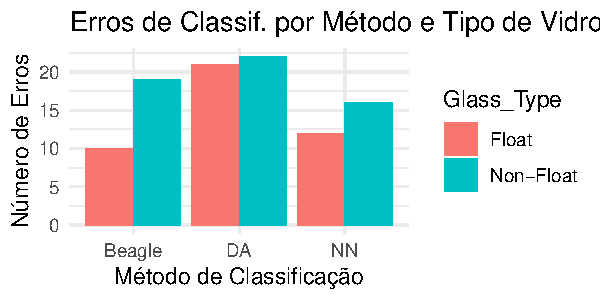
\includegraphics[keepaspectratio]{EstudoDirigido-GI_files/figure-latex/unnamed-chunk-2-1.pdf}}

\subsection{\texorpdfstring{Dimensionalidade dos Dados
}{Dimensionalidade dos Dados }}\label{dimensionalidade-dos-dados}

\begin{Shaded}
\begin{Highlighting}[]
\FunctionTok{dim}\NormalTok{(Glass)}
\end{Highlighting}
\end{Shaded}

\begin{verbatim}
## [1] 214  10
\end{verbatim}

Essa base de dados possui 214 amostras e 10 variáveis. E cada variável
representa uma característica química ou física dos fragmentos de vidro,
sendo a última variável uma classe, sendo o tipo do vidro.

\subsection{\texorpdfstring{Análise Estrutural das Variáveis
}{Análise Estrutural das Variáveis }}\label{anuxe1lise-estrutural-das-variuxe1veis}

Utilizando a função \texttt{str()} nos dá uma visão geral da base de
dados, como o tipo de cada variável e uma amostra de seus valores:

\begin{Shaded}
\begin{Highlighting}[]
\FunctionTok{str}\NormalTok{(Glass)}
\end{Highlighting}
\end{Shaded}

\begin{verbatim}
## 'data.frame':    214 obs. of  10 variables:
##  $ RI  : num  1.52 1.52 1.52 1.52 1.52 ...
##  $ Na  : num  13.6 13.9 13.5 13.2 13.3 ...
##  $ Mg  : num  4.49 3.6 3.55 3.69 3.62 3.61 3.6 3.61 3.58 3.6 ...
##  $ Al  : num  1.1 1.36 1.54 1.29 1.24 1.62 1.14 1.05 1.37 1.36 ...
##  $ Si  : num  71.8 72.7 73 72.6 73.1 ...
##  $ K   : num  0.06 0.48 0.39 0.57 0.55 0.64 0.58 0.57 0.56 0.57 ...
##  $ Ca  : num  8.75 7.83 7.78 8.22 8.07 8.07 8.17 8.24 8.3 8.4 ...
##  $ Ba  : num  0 0 0 0 0 0 0 0 0 0 ...
##  $ Fe  : num  0 0 0 0 0 0.26 0 0 0 0.11 ...
##  $ Type: Factor w/ 6 levels "1","2","3","5",..: 1 1 1 1 1 1 1 1 1 1 ...
\end{verbatim}

A partir dessa análise, podemos ver que todas as variáveis são do tipo
numérico, exceto a variável TYPE, que é um fator com 6 níveis,
representando as diferentes categorias de vidro.

\subsubsection{Distribuição das
Classes}\label{distribuiuxe7uxe3o-das-classes}

Agora, utilizando a função \texttt{table()}, nos permite ver o número de
amostras presentes em cada classe de vidro:

\begin{Shaded}
\begin{Highlighting}[]
\FunctionTok{table}\NormalTok{(Glass}\SpecialCharTok{$}\NormalTok{Type)}
\end{Highlighting}
\end{Shaded}

\begin{verbatim}
## 
##  1  2  3  5  6  7 
## 70 76 17 13  9 29
\end{verbatim}

Os resultados mostram a quantidade de amostras em cada 1 das 6 classes
de vidro, com isso podemos ver que as classes 1 e 2, correspondentes ao
vidro de construção de janelas, são as mais frequentes, enquanto as
outras classes têm uma quantidade menor de amostras.

\subsection{\texorpdfstring{Integridade da base de dados
}{Integridade da base de dados }}\label{integridade-da-base-de-dados}

Para verificar a integridade da base de dados e identificar se há
valores ausentes (NA), utilizamos de duas formas para essa verificação,
a função summary(glass), que fornece um resumo das variáveis, permitindo
identificar se há ou não valores NA.

\begin{Shaded}
\begin{Highlighting}[]
\FunctionTok{summary}\NormalTok{(Glass)}
\end{Highlighting}
\end{Shaded}

\begin{verbatim}
##        RI              Na              Mg              Al       
##  Min.   :1.511   Min.   :10.73   Min.   :0.000   Min.   :0.290  
##  1st Qu.:1.517   1st Qu.:12.91   1st Qu.:2.115   1st Qu.:1.190  
##  Median :1.518   Median :13.30   Median :3.480   Median :1.360  
##  Mean   :1.518   Mean   :13.41   Mean   :2.685   Mean   :1.445  
##  3rd Qu.:1.519   3rd Qu.:13.82   3rd Qu.:3.600   3rd Qu.:1.630  
##  Max.   :1.534   Max.   :17.38   Max.   :4.490   Max.   :3.500  
##        Si              K                Ca               Ba       
##  Min.   :69.81   Min.   :0.0000   Min.   : 5.430   Min.   :0.000  
##  1st Qu.:72.28   1st Qu.:0.1225   1st Qu.: 8.240   1st Qu.:0.000  
##  Median :72.79   Median :0.5550   Median : 8.600   Median :0.000  
##  Mean   :72.65   Mean   :0.4971   Mean   : 8.957   Mean   :0.175  
##  3rd Qu.:73.09   3rd Qu.:0.6100   3rd Qu.: 9.172   3rd Qu.:0.000  
##  Max.   :75.41   Max.   :6.2100   Max.   :16.190   Max.   :3.150  
##        Fe          Type  
##  Min.   :0.00000   1:70  
##  1st Qu.:0.00000   2:76  
##  Median :0.00000   3:17  
##  Mean   :0.05701   5:13  
##  3rd Qu.:0.10000   6: 9  
##  Max.   :0.51000   7:29
\end{verbatim}

E como segundo método, de uma forma mais direta, usamos a seguinte
função para mostrar se há algum valor NA nesta base:

\begin{Shaded}
\begin{Highlighting}[]
\FunctionTok{sum}\NormalTok{(}\FunctionTok{is.na}\NormalTok{(Glass))}
\end{Highlighting}
\end{Shaded}

\begin{verbatim}
## [1] 0
\end{verbatim}

Após essa verificação, pode-se dizer que não há dados ausentes na base
de dados, ou seja todas as amostras desta base estão completas.
Portanto, não é necessário retirar nenhuma amostra.

\subsubsection{Balanceamento dos dados}\label{balanceamento-dos-dados}

Para identificar o balanceamento da base de dados, calculamos a
porcentagem de cada classe em relação ao total de amostras usando a
função prop.table. A fórmula utilizada foi:

\begin{Shaded}
\begin{Highlighting}[]
\FunctionTok{round}\NormalTok{(}\FunctionTok{prop.table}\NormalTok{(}\FunctionTok{table}\NormalTok{(Glass}\SpecialCharTok{$}\NormalTok{Type)) }\SpecialCharTok{*} \DecValTok{100}\NormalTok{, }\DecValTok{2}\NormalTok{)}
\end{Highlighting}
\end{Shaded}

\begin{verbatim}
## 
##     1     2     3     5     6     7 
## 32.71 35.51  7.94  6.07  4.21 13.55
\end{verbatim}

E com base nos resultados, podemos ver um desequilíbrio entre as
classes, com a classe mais frequente representando 32,71\% das amostras,
enquanto a classe menos frequente representa apenas 4,21\%, pOr isso
sugere que os dados não estão balanceados.

\subsection{\texorpdfstring{Problemas de Regressão
}{Problemas de Regressão }}\label{problemas-de-regressuxe3o}

Para problemas de regressão, devemos calcular as médias e desvios-padrão
de todas as variáveis numéricas. Para isso utilizamos o código utilizado
para essa análise logo abaixo:

\begin{verbatim}
##    Média Desvio_Padrão
## RI  1.52          0.00
## Na 13.41          0.82
## Mg  2.68          1.44
## Al  1.44          0.50
## Si 72.65          0.77
## K   0.50          0.65
## Ca  8.96          1.42
## Ba  0.18          0.50
## Fe  0.06          0.10
\end{verbatim}

\subsubsection{Análise de Outliers}\label{anuxe1lise-de-outliers}

Os outliers podem influenciar significativamente a análise de dados,
especialmente em problemas de classificação. Para identificar os
outliers na base de dados, criamos gráficos de boxplot para cada uma das
variáveis, que podem ajudar a visualizar a distribuição dos dados,
identificando valores atípicos (outliers) que se encontram fora dos
limites interquartis.

\begin{Shaded}
\begin{Highlighting}[]
\NormalTok{numeric\_vars }\OtherTok{\textless{}{-}}\NormalTok{ Glass[, }\FunctionTok{sapply}\NormalTok{(Glass, is.numeric)]}
\FunctionTok{par}\NormalTok{(}\AttributeTok{mfrow =} \FunctionTok{c}\NormalTok{(}\DecValTok{3}\NormalTok{, }\DecValTok{3}\NormalTok{))  }
\ControlFlowTok{for}\NormalTok{ (i }\ControlFlowTok{in} \DecValTok{1}\SpecialCharTok{:}\FunctionTok{ncol}\NormalTok{(numeric\_vars)) \{}
  \FunctionTok{boxplot}\NormalTok{(numeric\_vars[, i], }\AttributeTok{main =} \FunctionTok{colnames}\NormalTok{(numeric\_vars)[i], }\AttributeTok{col =} \StringTok{"lightblue"}\NormalTok{, }\AttributeTok{border =} \StringTok{"blue"}\NormalTok{)}
\NormalTok{\}}
\end{Highlighting}
\end{Shaded}

\pandocbounded{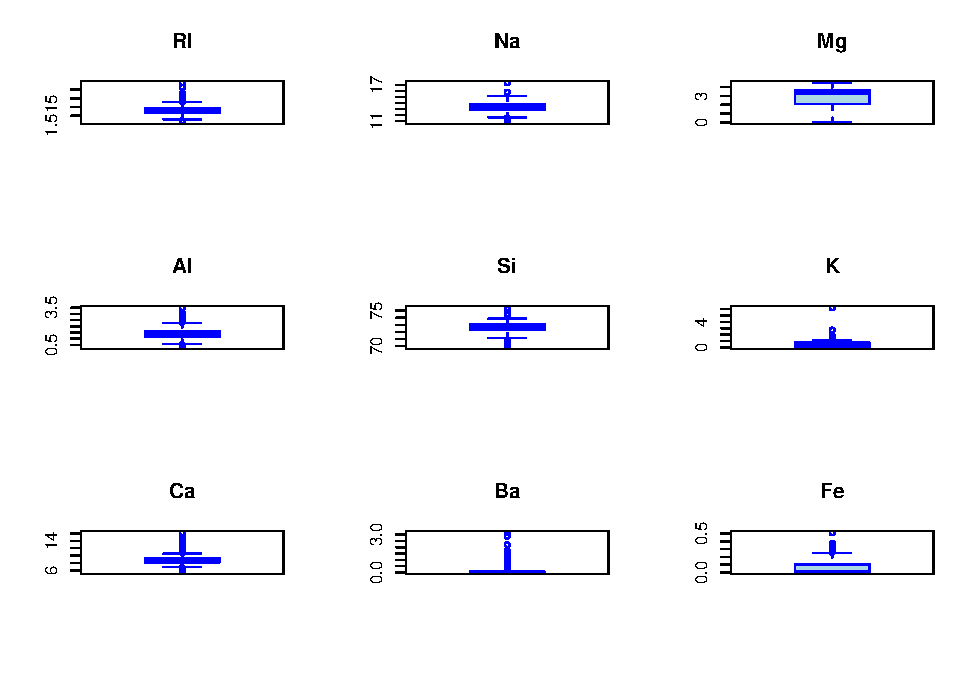
\includegraphics[keepaspectratio]{EstudoDirigido-GI_files/figure-latex/unnamed-chunk-10-1.pdf}}

Esse código cria boxplots para cada variável numérica da base de dados,
o que facilita a identificação de valores fora da faixa esperada.
Valores que estão além dos limites superior e inferior do boxplot
(geralmente 1,5 vezes o intervalo interquartil) são considerados
outliers.

Sendo assim, os gráficos mostram que algumas variáveis apresentam
outliers evidentes, como \textbf{Sódio (Na)} e \textbf{Magnésio (Mg)}
possuem valores que claramente se afastam da maioria das amostras.

\subsection{\texorpdfstring{Análise Descritiva das Variáveis
}{Análise Descritiva das Variáveis }}\label{anuxe1lise-descritiva-das-variuxe1veis}

Na análise descritiva, faremos uma análise descritiva para cada
variável, incluindo os valores mínimo, máximo, média e desvio padrão,
separando os dados por classes. Aqui, estamos interessados nas
características numéricas do conjunto de dados em função da variável de
classe (o tipo de vidro). Como podemos ver logo abaixo:

\begin{verbatim}
## # A tibble: 6 x 37
##   Type  RI_Min RI_Max RI_Média `RI_Desvio Padrão` Na_Min Na_Max Na_Média
##   <fct>  <dbl>  <dbl>    <dbl>              <dbl>  <dbl>  <dbl>    <dbl>
## 1 1       1.51   1.53     1.52            0.00227   12.4   14.8     13.2
## 2 2       1.51   1.53     1.52            0.00380   10.7   14.9     13.1
## 3 3       1.52   1.52     1.52            0.00192   12.2   14.3     13.4
## 4 5       1.51   1.52     1.52            0.00335   11.0   14.0     12.8
## 5 6       1.51   1.52     1.52            0.00312   13.8   17.4     14.6
## 6 7       1.51   1.52     1.52            0.00255   12.0   15.8     14.4
## # i 29 more variables: `Na_Desvio Padrão` <dbl>, Mg_Min <dbl>, Mg_Max <dbl>,
## #   Mg_Média <dbl>, `Mg_Desvio Padrão` <dbl>, Al_Min <dbl>, Al_Max <dbl>,
## #   Al_Média <dbl>, `Al_Desvio Padrão` <dbl>, Si_Min <dbl>, Si_Max <dbl>,
## #   Si_Média <dbl>, `Si_Desvio Padrão` <dbl>, K_Min <dbl>, K_Max <dbl>,
## #   K_Média <dbl>, `K_Desvio Padrão` <dbl>, Ca_Min <dbl>, Ca_Max <dbl>,
## #   Ca_Média <dbl>, `Ca_Desvio Padrão` <dbl>, Ba_Min <dbl>, Ba_Max <dbl>,
## #   Ba_Média <dbl>, `Ba_Desvio Padrão` <dbl>, Fe_Min <dbl>, Fe_Max <dbl>, ...
\end{verbatim}

Essa tabela mostra como os valores de cada variável variam entre as
classes. A partir dela, podemos identificar como as propriedades
químicas distinguem os diferentes tipos de vidro.

\subsubsection{Gráficos das Variáveis por
Classe}\label{gruxe1ficos-das-variuxe1veis-por-classe}

Para visualizar melhor como as variáveis se comportam em relação às
classes de vidro, podemos usar gráficos de dispersão, onde mapeamos cada
variável em relação à classe.

\pandocbounded{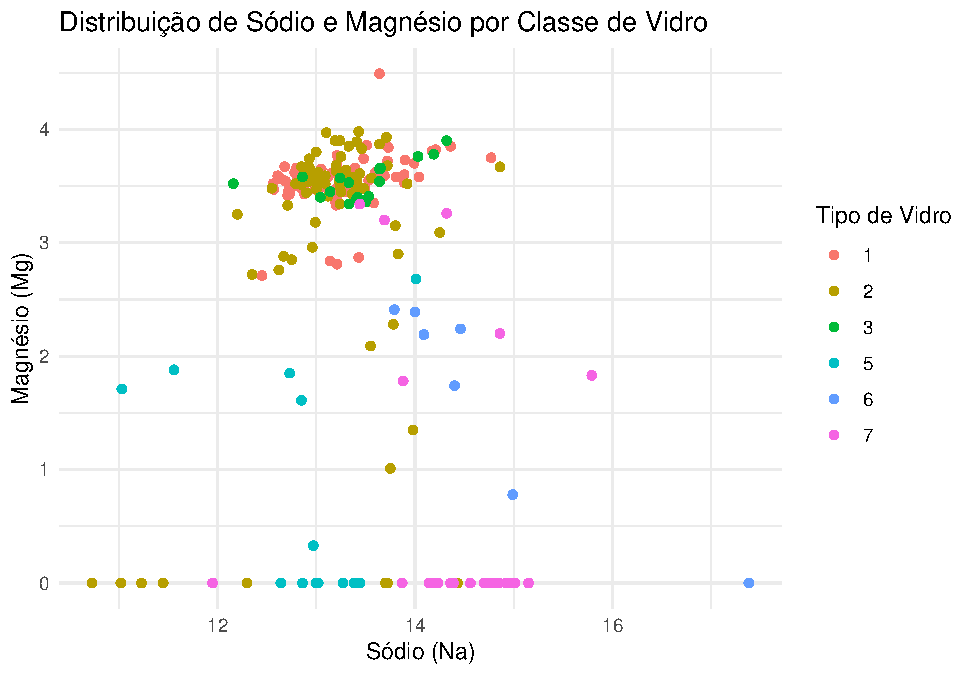
\includegraphics[keepaspectratio]{EstudoDirigido-GI_files/figure-latex/unnamed-chunk-12-1.pdf}}
\pandocbounded{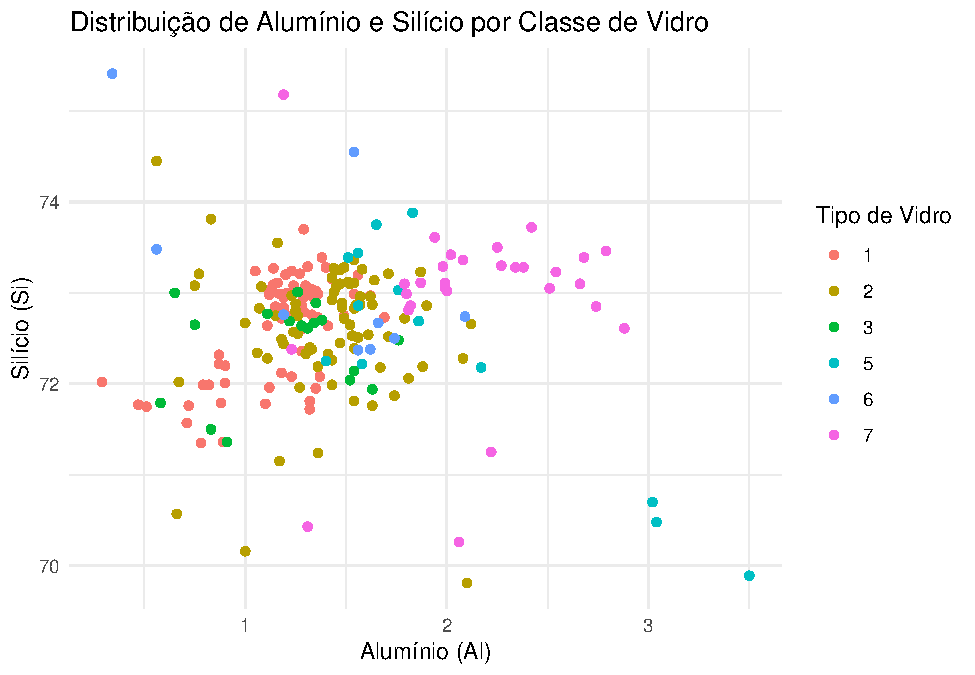
\includegraphics[keepaspectratio]{EstudoDirigido-GI_files/figure-latex/unnamed-chunk-12-2.pdf}}

Esses gráficos de dispersão mostram como algumas variáveis se agrupam
por classe, o que sugere que as propriedades químicas são bons
indicadores para a classificação do vidro.

E os resultados mostram que variáveis como \textbf{Na}, \textbf{Mg},
\textbf{Al} e \textbf{Si} têm padrões distintos que ajudam a diferenciar
as classes, por isso essa visualização facilita a compreensão de como
cada amostra está distribuída e como as classes se separam com base nas
características químicas.

\subsection{\texorpdfstring{Análise de Correlação
}{Análise de Correlação }}\label{anuxe1lise-de-correlauxe7uxe3o}

A correlação entre as variáveis numéricas da base de dados pode ajudar a
entender como cada característica está relacionada com a classe de
vidro, por isso, temos que calcular a matriz de correlação e visualizar
um gráfico de correlação, como abaixo:

\pandocbounded{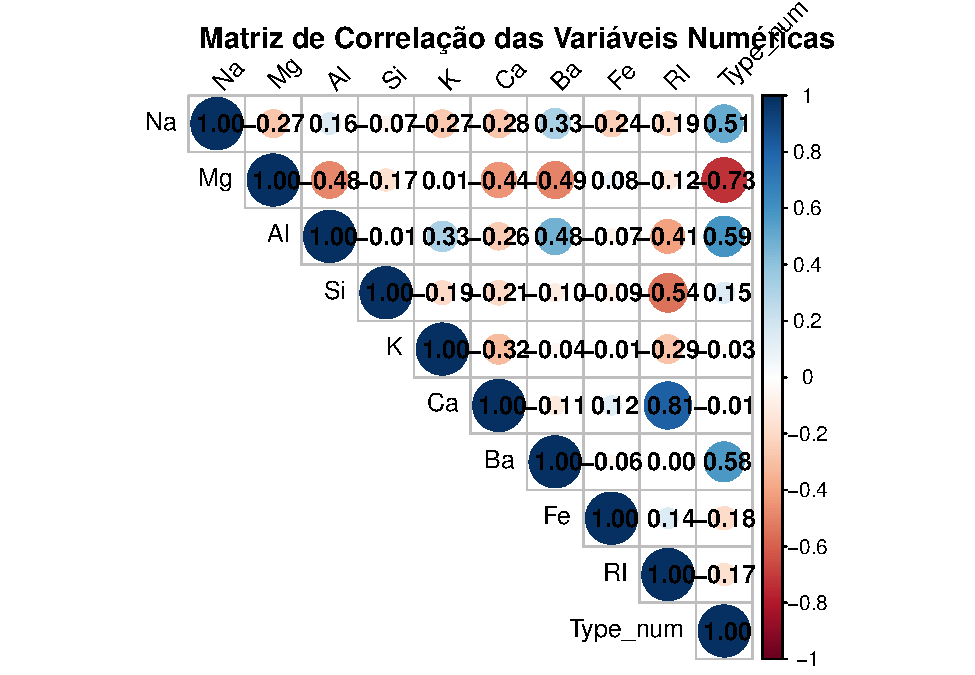
\includegraphics[keepaspectratio]{EstudoDirigido-GI_files/figure-latex/unnamed-chunk-13-1.pdf}}

Neste gráfico podemos perceber que a matriz de correlação acima mostra
como cada variável numérica está relacionada tanto entre si quanto com a
classe de vidro e os coeficientes de correlação variam entre -1 e 1,
onde valores próximos de 1 indicam uma correlação positiva forte, e
valores próximos de -1 indicam uma correlação negativa forte.

E a variável de classe \textbf{TYPE} tem correlação com várias das
variáveis químicas, como \textbf{Na}, \textbf{Mg}, e \textbf{Si},
sugerindo que essas variáveis são importantes na distinção dos tipos de
vidro. Nos permitindo identificar quais variáveis têm maior influência
sobre a classificação do vidro e podem ser boas opções para futuras
classificações.

\subsection{\texorpdfstring{Pré-processamento e Padrões Esperados
}{Pré-processamento e Padrões Esperados }}\label{pruxe9-processamento-e-padruxf5es-esperados}

Com essa análise identificamos que a base de dados não possui dados
ausentes, mas apresenta desequilíbrio nas classes. Portanto, isso requer
a aplicação de técnicas de balanceamento, como oversampling ou
undersampling. Além disso, seria interessante testar normalizações nas
variáveis numéricas para garantir que as diferenças nas escalas dos
dados não influenciem negativamente os modelos.

E sobre os padrãos, espera-se encontrar padrões relacionados à
composição química dos vidros que ajudem a distinguir os diferentes
tipos de vidro e a mineração de dados pode explorar essas
características químicas para fornecer uma classificação precisa,
ajudando em contextos forenses como ditos.

\subsection{\texorpdfstring{Estudos de artigos sobre a base de dados
}{Estudos de artigos sobre a base de dados }}\label{estudos-de-artigos-sobre-a-base-de-dados}

\begin{table}
\centering
\caption{\label{tab:unnamed-chunk-14}}
\centering
\fontsize{10}{12}\selectfont
\begin{tabu} to \linewidth {>{\raggedright}X>{\raggedright}X>{\raggedright}X>{\raggedright}X}
\hline
Titulo & Estatistica\_Descritiva & Pre\_Processamento & Objetivo\\
\hline
Exploring the Power and Practical Applications of K-Nearest Neighbours (KNN) in Machine Learning & A base de dados UCI Glass Identification possui dez propriedades, uma das quais é o ID, que foi removido. Existem sete valores discretos na resposta do tipo de vidro. Os atributos incluem RI (índice de refração), Na (Sódio), Si (Silício), Mg (Magnésio), entre outros, que são medidos em peso percentual. & O pré-processamento dos dados foi conduzido para verificar se havia valores ausentes, e o conjunto de dados foi transformado em formato ARFF. A validação cruzada estratificada de 10 vezes foi usada para reduzir a variância e fornecer uma estimativa precisa do desempenho. & O objetivo do estudo foi classificar amostras de vidro como 'float' ou não 'float', utilizando diferentes abordagens, como o algoritmo de K-vizinhos mais próximos (KNN), árvore de decisão C4.5 e K-Means. O estudo foi motivado por investigações criminais, onde a identificação correta do vidro é crucial.\\
\hline
Glass recognition as a cutting-edge machine learning approach for identification and classification & A base de dados contém 214 observações coletadas no Home Office Forensic Science Laboratory, Birmingham. As variáveis incluem componentes químicos como Sódio (Na), Magnésio (Mg), Cálcio (Ca), Bário (Ba), entre outros, além do índice de refração (RI). A classe dos vidros é representada por sete tipos, como janelas de edifícios (float e non-float) e faróis. & O pré-processamento incluiu limpeza dos dados para corrigir erros, seleção de variáveis relevantes e visualização para identificar outliers e padrões. Técnicas de normalização e redução de dimensionalidade foram aplicadas antes do treinamento dos modelos de aprendizado de máquina. & O objetivo do estudo foi desenvolver um modelo de identificação e classificação de vidros usando redes neurais profundas e algoritmos de árvore de decisão, visando categorizar corretamente os diferentes tipos de vidro em investigações criminais e processos de tomada de decisão.\\
\hline
\end{tabu}
\end{table}

\end{document}
